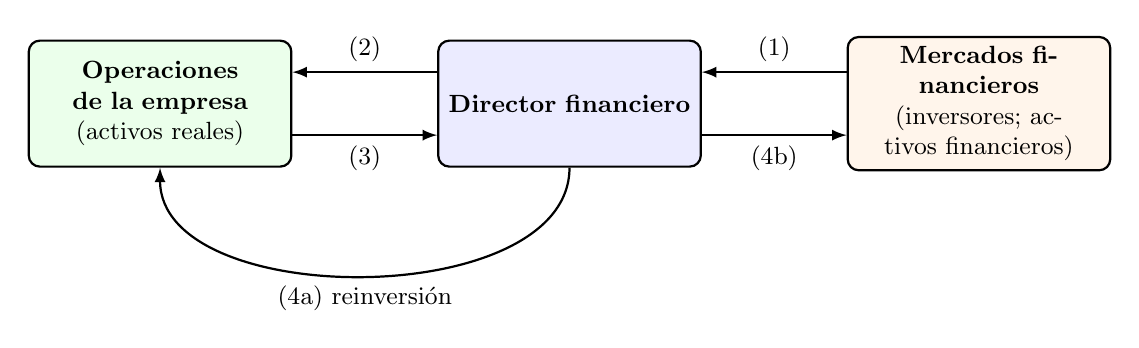
\begin{tikzpicture}[>=latex, font=\small,
  caja/.style={draw, thick, rounded corners, align=center, minimum height=1.6cm, text width=3.1cm, fill=#1!8},
  caja/.default=gray]
  \node[caja=green] (op) at (0,0) {\textbf{Operaciones de la empresa}\\(activos reales)};
  \node[caja=blue] (df) at (5.2,0) {\textbf{Director financiero}};
  \node[caja=orange] (mf) at (10.4,0) {\textbf{Mercados financieros}\\(inversores; activos financieros)};
  \draw[->, thick] ([yshift=4mm]mf.west) -- node[above] {(1)} ([yshift=4mm]df.east);
  \draw[->, thick] ([yshift=-4mm]df.east) -- node[below] {(4b)} ([yshift=-4mm]mf.west);
  \draw[->, thick] ([yshift=4mm]df.west) -- node[above] {(2)} ([yshift=4mm]op.east);
  \draw[->, thick] ([yshift=-4mm]op.east) -- node[below] {(3)} ([yshift=-4mm]df.west);
  \draw[->, thick] (df.south) to[out=-90, in=-90, looseness=0.9] node[below] {(4a) reinversión} (op.south);
\end{tikzpicture}
